\documentclass[11pt]{article}
\usepackage{color}
\usepackage[usenames,dvipsnames,svgnames,table]{xcolor}
\definecolor{dark-red}{rgb}{0.7,0.1,0.1} 
\definecolor{dark-blue}{rgb}{0,0,0.7} 
\usepackage[linkcolor=dark-red,
            colorlinks=true,
            urlcolor=dark-blue,
            pdfstartview={XYZ null null 1.00},
            pdfauthor={Gaurav Sood, gsood07@gmail.com; Andy Guess, a.guess@columbia.edu},
            citecolor=dark-red,
            bookmarks=false,
            pdfborder={0 0 0},
            pdftitle={Quantitative Discipline}]{hyperref}
            
\usepackage{amsfonts,amssymb,amsbsy,amsmath,amsxtra}

\usepackage{indentfirst}
\usepackage{setspace} % To set line spacing
\usepackage{multirow}

\usepackage{verbatim}

\usepackage[multiple]{footmisc}
\usepackage{fancyvrb}

\usepackage{longtable}

\usepackage[margin=1in]{geometry}
\usepackage{graphicx}

\raggedright
\parindent=1.5em % <- or whatever indent you want

\begin{comment}
	
	tools::texi2dvi("cricket.tex", pdf=TRUE, clean=TRUE)	

\end{comment}

\begin{document}
\title{\vspace{-2.0cm}\normalsize{\textbf{Fairly Random: Impact of Winning the Toss on the Probability of Winning}}}
\author{Gaurav Sood\thanks{\href{mailto:gsood07@gmail.com}{\texttt{gsood07@gmail.com}}.} \and Derek Willis\thanks{\href{mailto:dwillis@gmail.com}{\texttt{dwillis@gmail.com}}.}}
\maketitle
\doublespacing



In many cricket matches, it is claimed that there is a clear advantage to bowling (batting) first. The advantage is pointed to by commentators, and by captains of the competing teams in the pre-toss interview. And sometimes in the post-match interview.

The opportunity to bowl or bat first is decided by a coin toss. While this method of deciding on who is advantaged is fair on average, the system isn't fair in any one game. At first glance, the imbalance seems inevitable. After all someone has to bat first. One can, however, devise a baseball like system where short innings are interspersed. If that violates the nature of the game too much, one can easily create pitches that don't deteriorate appreciably over the course of a game. Or, one can come up with an estimate of the advantage and adjust scores accordingly (something akin to an adjustment issued when matches are shortened due to rain).

But before we move to seriously consider these solutions, one may ask about the evidence.

Data are from nearly five thousand one-day international matches.

The team that wins the toss wins the match approximately 49.3\% of the times. With 5335 matches, we cannot rule out that the true proportion is 50\%. Thus, counter to intuition, the effect of winning the toss is, on average, at best minor. This may be so because it is impossible to predict well in advance the advantage of bowling or batting first. Or it may simply be because teams are bad at predicting it, perhaps because they use bad heuristics.

\begin{figure}[htbp]
\centering
\caption{Proportion of Matches Won Minus Matches Lost After Winning the Toss}
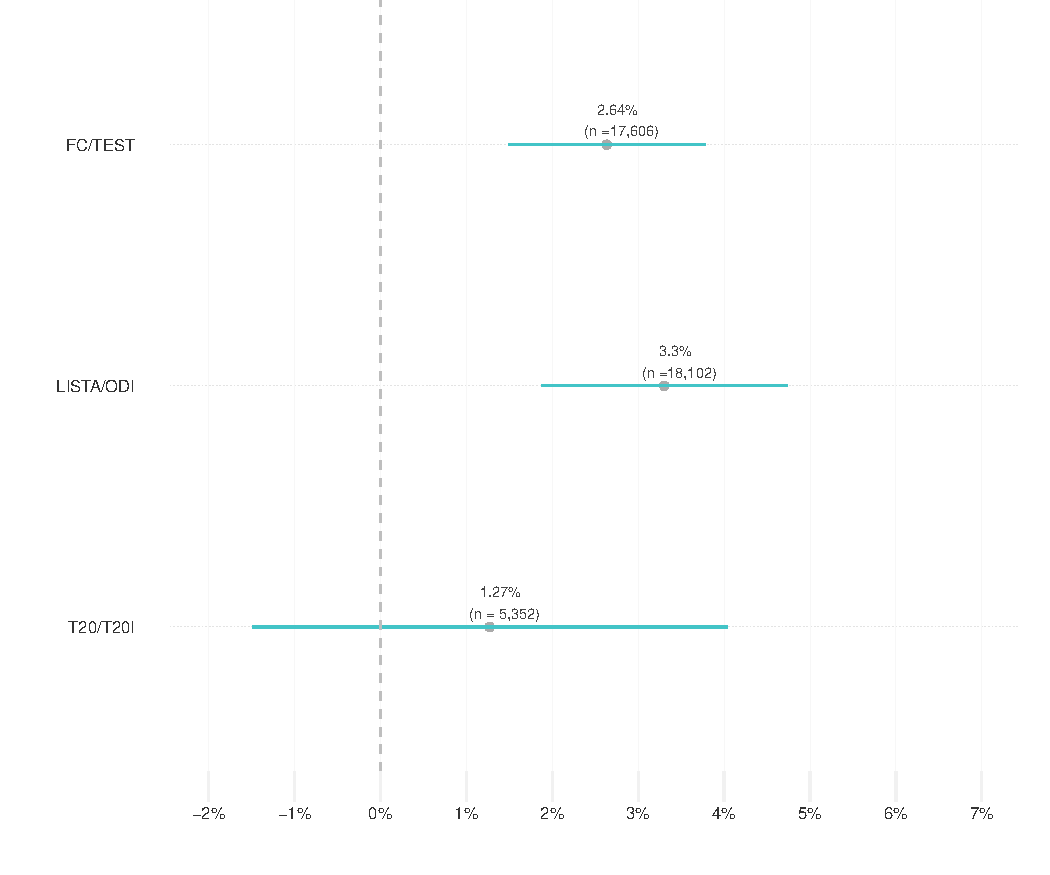
\includegraphics[scale=.75]{../figs/winbyType.pdf}
\label{fig:summary}
\end{figure}

No effects across the entire sample may hide some subgroup effects. It is often claimed that toss is more crucial in day and night matches, due to dew and lower visibility of the white ball under lights. And data show as much.

It may well be the case that toss is more important in tests than one-day matches.

\begin{figure}[htbp]
\centering
\caption{Proportion of Matches Won Minus Matches Lost After Winning the Toss}
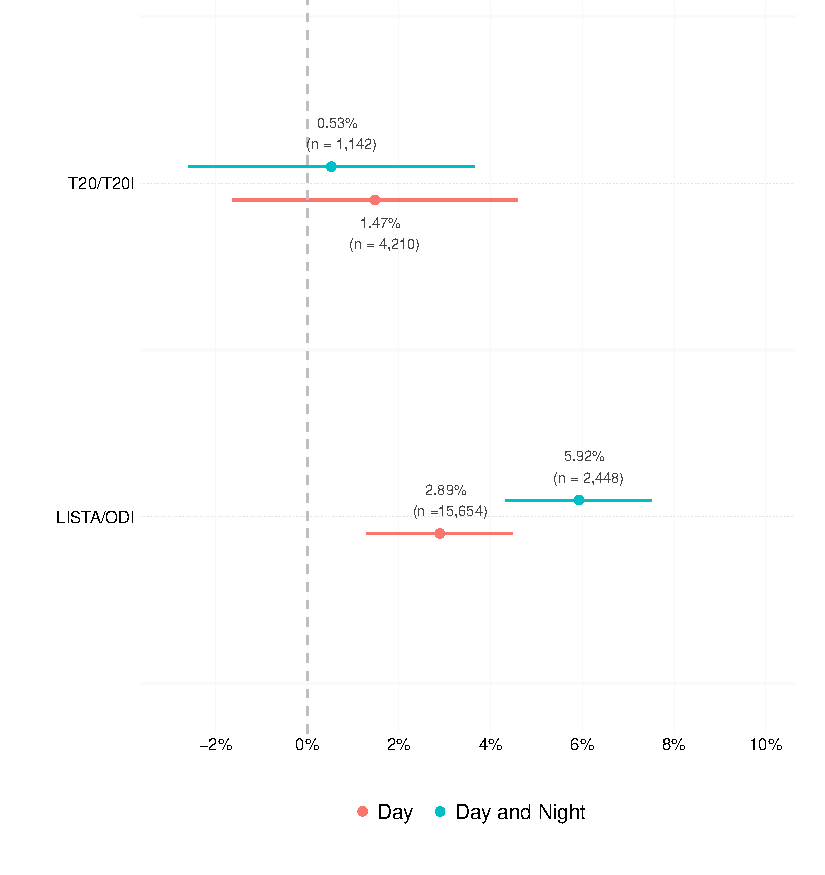
\includegraphics[scale=.75]{../figs/winbyDayNight.pdf}
\label{fig:summary}
\end{figure}


\begin{figure}[htbp]
\centering
\caption{Proportion of Matches Won Minus Matches Lost After Winning the Toss}
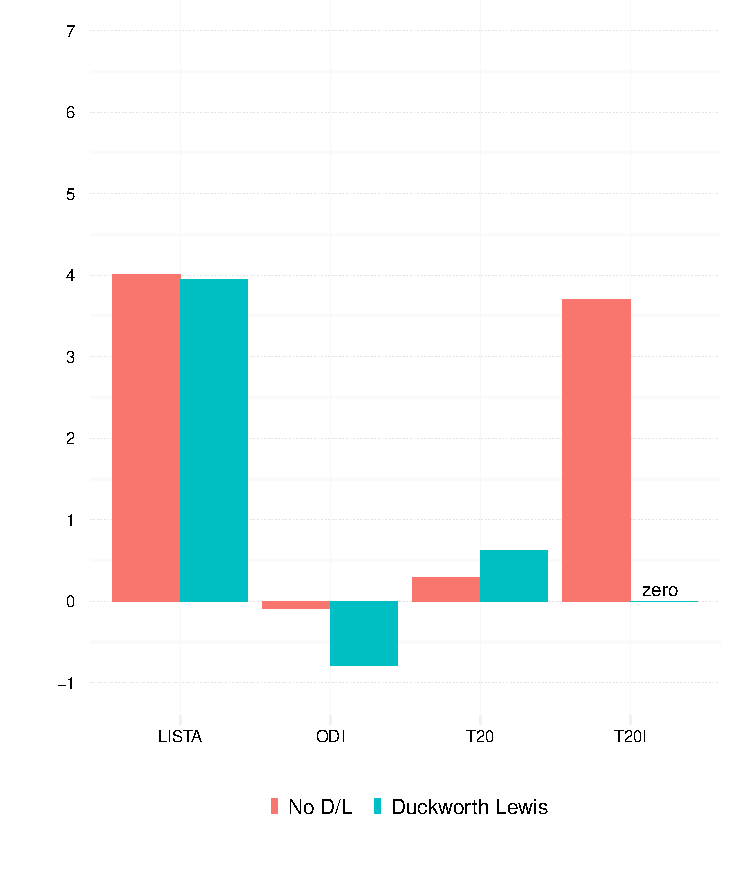
\includegraphics[scale=.75]{../figs/winbyDL.pdf}
\label{fig:summary}
\end{figure}

\end{document}